\documentclass[12pt,onecolumn,a4paper,fleqn]{article}
\usepackage[top=1in, bottom=1in, left=0.75in, right=0.75in]{geometry}
\usepackage{epsfig,graphicx,subfigure,amsthm,amsmath}
\usepackage[table,xcdraw,svgnames]{xcolor}
\usepackage{setspace}
\usepackage{mathtools}
\usepackage{fancyhdr}
\usepackage{sidecap}
\usepackage{tikz}
\usepackage{pgfplots}
\usetikzlibrary{decorations.pathreplacing}
\usepackage{relsize}
\usepackage{color,xcolor}
\usepackage[framed,numbered]{matlab-prettifier}
\usepackage{float}
\usepackage{enumerate}
\usepackage{booktabs}
\usepackage{setspace}
\usepackage{datetime}
\usepackage{hyperref}
\usepackage{xepersian}

\hypersetup{
	colorlinks=true,
	urlcolor=blue!70!black,
	linkcolor=blue
}


\settextfont[Path=fonts/,BoldFont={ZarBd.ttf},BoldFeatures={Scale=0.9}]{BZar.ttf}

%\DeclarePairedDelimiter\ceil{\lceil}{\rceil}
%\DeclarePairedDelimiter\floor{\lfloor}{\rfloor}

%\definecolor{vgreen}{RGB}{104,180,104}
%\definecolor{vblue}{RGB}{49,49,255}
%\definecolor{vorange}{RGB}{255,143,102}


% title page template
\newcommand{\heading}[1]
{
	\begin{center}
		\begin{huge}
			\textbf{
				به نام خدا\\
			}
		\end{huge}
		
		\vspace*{1.5cm}
		
\includegraphics[scale=0.9]{source/sharif_logo.png}\\
		\vspace*{0.5cm}
		\begin{Large}
			\textbf{
				دانشگاه صنعتی شریف\\
				\vspace*{0.25cm}
				دانشکده مهندسی کامپیوتر\\
			}
		\end{Large}
		\vspace*{3cm}
		\begin{huge}
			\textbf{
				آزمایشگاه معماری کامپیوتر\\
				\vspace*{0.75cm}
			}
		\end{huge}
		
		\begin{Large}
			\textbf{
				آزمایش هفتم:\\
				#1\\
			}
		\end{Large}
		
		\noindent\rule[1ex]{\linewidth}{1pt}\\
		\vspace*{0.5cm}
		\begin{table}[H]
			\centering
			\begin{tabular}{|c|c|}
				\hline
				\multicolumn{2}{|c|}{\textbf{اطلاعات تیم}}
				\\ \hline
				\textbf{نام اعضا} & \textbf{شماره دانشجویی}
				\\ \hline
				متین داغیانی & 98106456
				\\ \hline
				بردیا محمدی & 98171104
				\\ \hline
				محمدجواد هزاره & 98101074
				\\ \hline 
			\end{tabular}
		\end{table}
		\begin{Large}				
			\vspace*{0.75cm}
			\textbf{
				زمستان 1400
			}
		\end{Large}			
	\end{center}
}

\pagestyle{fancy}
\fancyhf{}
\rhead{\textbf{آزمایشگاه معماری کامپیوتر}}
%%--------------------[should change]---------------------
\chead{\textbf{گزارش آزمایش هفتم}}
%%--------------------[should change]---------------------
\lhead{\textbf{\nouppercase{\rightmark}}}
\cfoot{({\thepage})}
\renewcommand{\headrulewidth}{1pt}
\renewcommand{\footrulewidth}{1pt}
\renewcommand{\sectionmark}[1]{\markright{#1}}
\renewcommand{\subsectionmark}[1]{\markright{#1}}
%\newdateformat{monthyeardate}{%
	%	\monthname[\THEMONTH], \THEYEAR}

\onehalfspacing
\begin{document}
	%%% title pages
	\large
	\begin{titlepage}
		\heading{استفاده از حافظه داده و دستورات پرش}
		\thispagestyle{empty}
	\end{titlepage}	
	\pagebreak
	
	%%% contents page
	\tableofcontents
	\thispagestyle{empty}
	\pagebreak
	
	%%% figures page
	\listoffigures
	\thispagestyle{empty}
	\pagebreak
	
	%%% main document
	\section{هدف آزمایش}
	در این آزمایش قصد داریم تا با اضافه کردن امکانات پرش و خواندن داده از حافظه، مدار طراحی شده در آزمایش شماره شش را تکمیل کرده و در نهایت به یک کامپیوتر ساده با معماری \lr{Harvard}دست یابیم. به همین جهت در گام اول یک \lr{RAM} با گنحایش 32 بایت را به مدار اضافه می کنیم و در نتیجه امکان ذخیره مقادیر بینابینی را در این حافظه پیدا خواهیم کرد. هم چنین در ادامه امکان استفاده از دستورات پرش شرطی و غیر شرطی را فراهم خواهیم کرد. در شکل \ref{fig:1} دیاگرام بلوکی مدار نهایی را مشاهده می کنید:
	\begin{figure}[H]
		\centering
		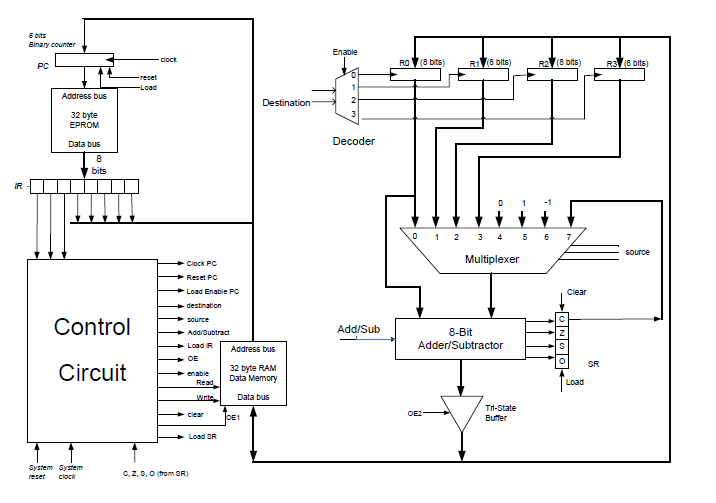
\includegraphics[width=0.8\textwidth]{source/1.png}
		\caption{بلوک دیاگرام سیسیتم}
		\label{fig:1}
	\end{figure}
	همان طور که در شکل مشخص است، یک حافظه داده با ظرفیت 32 بایت اضافه شده است که امکان ذخیره و بازیابی داده‌ها را فراهم می‌کند. این حافظه از طریق سیگنال‌های کنترلی \lr{Read} و \lr{Write} با واحد کنترل در ارتباط است. هم‌چنین در قسمت جریان داده، رجیسترهای \lr{flag} اضافه شده‌اند که برای دستورات پرش شرطی مورد ارزیابی قرار می‌گیرند.
	
	نمای کلی مدار پیاده‌سازی شده در شکل \ref{fig:2} آمده است.
	\begin{figure}[H]
		\centering
		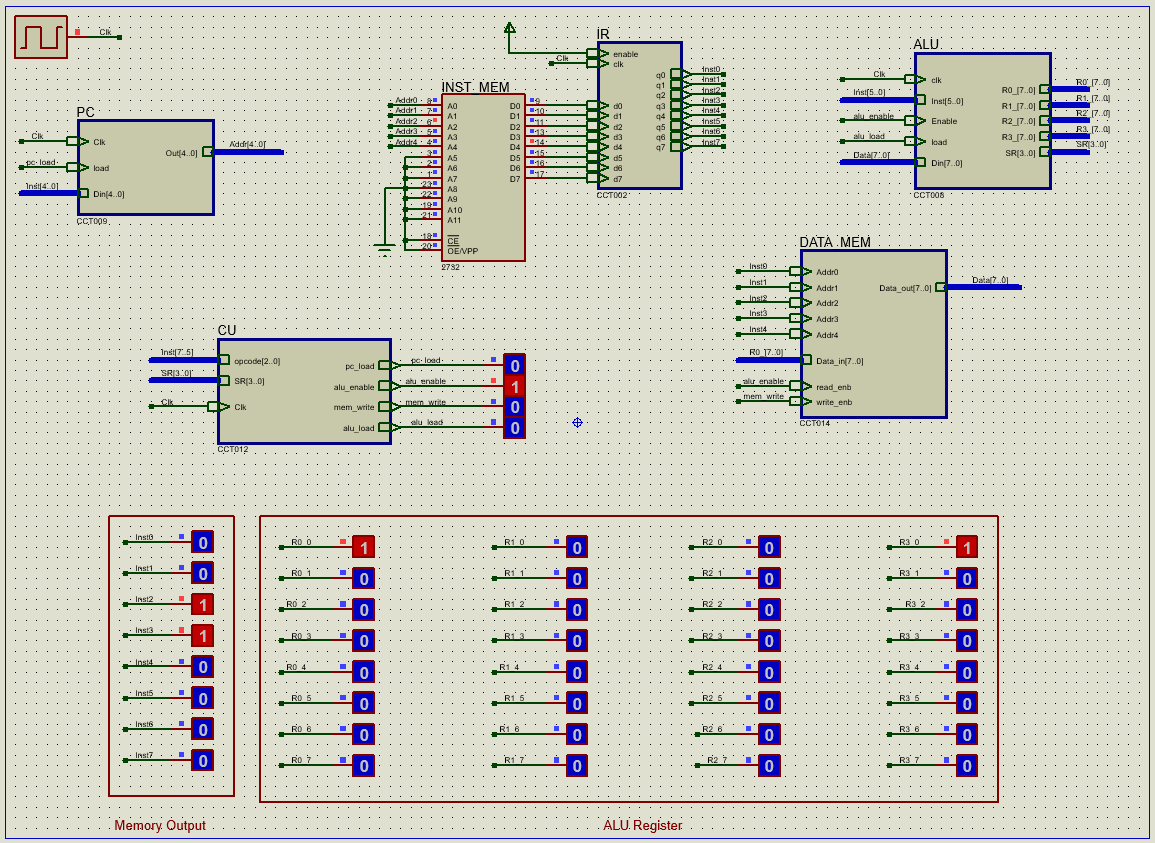
\includegraphics[width=0.9\textwidth]{source/circuit.png}
		\caption{نمای کلی سیستم پیاده سازی شده}
		\label{fig:2}
	\end{figure}
	
	%---------------------------------------------------------------------------------
	\pagebreak
	\section{مراحل طراحی و پیاده‌سازی مدار}
	\subsection {ماژول‌های مورد نیاز و شروع به کار مدار}
	همانطور که در شکل \ref{fig:1} مشخص است، برای کنترل سیگنال‌های کنترلی به واحد \lr{CU} نیاز داریم. به علاوه با توجه به اضافه شدن دستورات پرش شرطی و غیر شرطی ماژول \lr{PC} نسبت به آزمایش قبلی به روز شده است. هم چنین ماژول دیگری به نام \lr{DATA\_MEM} نیز برای ذخیره و بازیابی داده‌ها در نظر گرفته شده است. در ادامه به بررسی دقیق تر هر ماژول خواهیم پرداخت.
	\subsection{ماژول \lr{PC}}
	\begin{figure}[H]
		\centering
		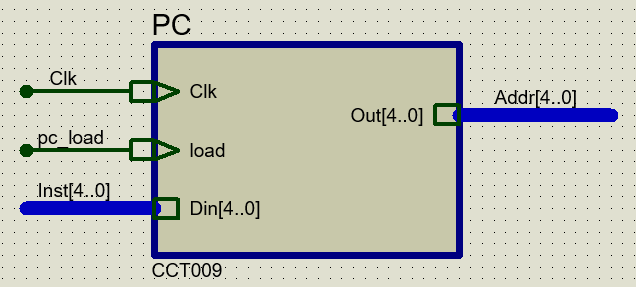
\includegraphics[width=0.55\textwidth]{source/pc_interface.png}
		\caption{ماژول \lr{PC}}
		\label{fig:3}
	\end{figure}
	برای پیاده سازی این ماژول از یک شمارنده بالا/پایین دودویی استفاده شده است که امکان لود موازی را نیز داراست (تراشه شماره 4516). ورودی‌های آن سیگنال
	\lr{pc\_load}
	،
	\lr{Inst[4..0]}
	و
	\lr{Clk}
	هستند که در شکل مشخص است. طراحی داخلی این ماژول را در شکل \ref{fig:pc-inner} می‌توان دید.
	\begin{figure}[H]
		\centering
		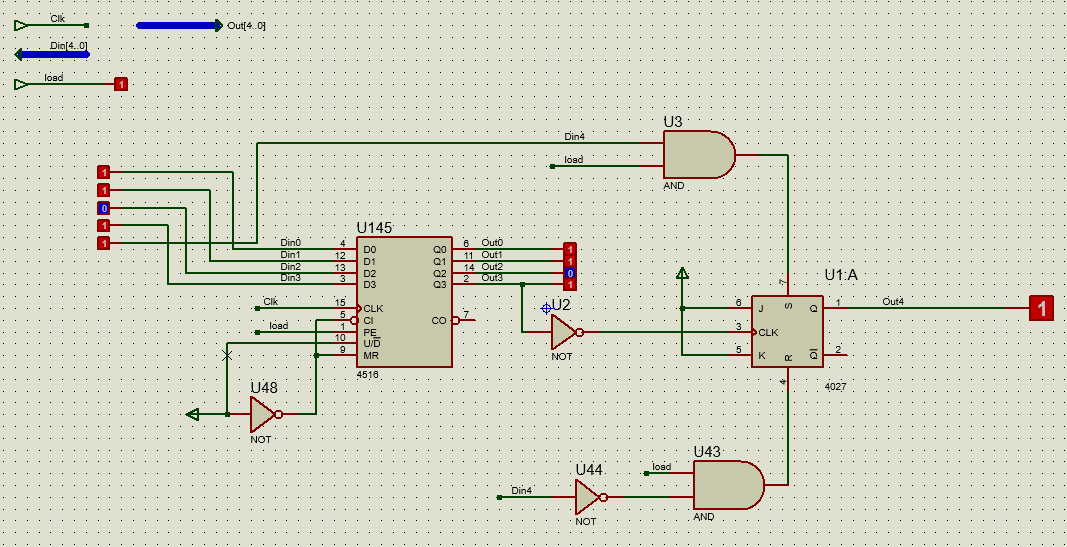
\includegraphics[width=0.8\textwidth]{source/pc_inner.png}
		\caption{طراحی داخلی ماژول \lr{PC}}
		\label{fig:pc-inner}
	\end{figure}
	همانطور که در شکل دیده می‌شود، برای طراحی این مدار از یک شمارنده‌ی ۴بیتی (تراشه ‌\lr{4516}) استفاده شده است. این تراشه قابلیت بارگذاری موازی را نیز داراست که به چهار ورودی آن، چهار بیت کم‌ارزش ورودی ماژول داده شده است. برای شمارش بیت پنج، همانطور که در شکل دیده می‌شود با تغیر بیت چهارم خروجی، بیت پنج کلاک خورده و تغییر می‌کند. برای ست کردن این بیت نیز مطابق شکل از ورودی‌های \lr{set} و \lr{reset} فلیپ‌فلاپ استفاده شده است. با $1$ شدن سیگنال ورودی \lr{load}، ورودی در خروجی بارگذاری شده و شمارش از آن عدد به بالا ادامه پیدا خواهد کرد.
	\subsection{ماژول \lr{INST\_MEM} و \lr{IR}}
	ماژول 
	\lr{INST\_MEM}
	نسبت به آزمایش قبلی تغییری نکرده است. اما ماژول
	\lr{IR}
	در این آزمایش به مدار اضافه شده که همان رجیستر شامل دستورالعمل است.
	\begin{figure}[H]
		\centering
		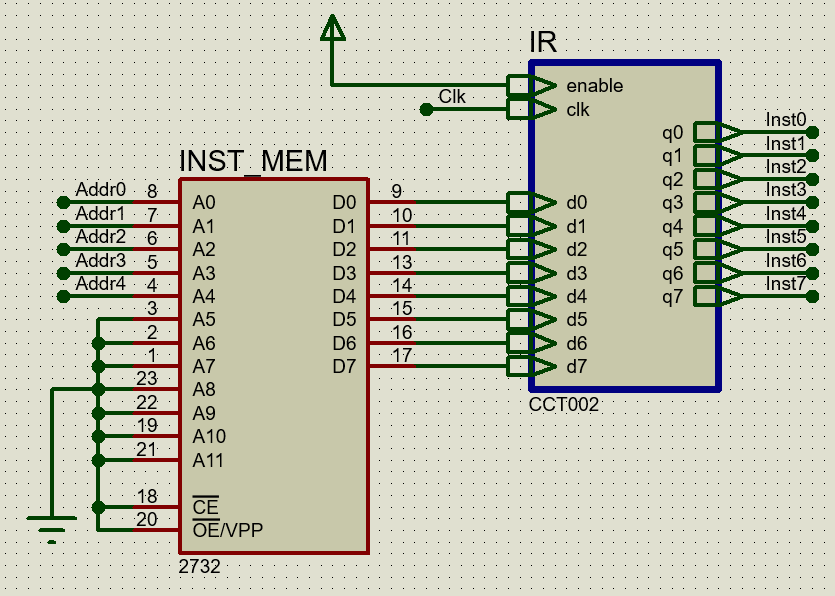
\includegraphics[width=0.48\textwidth]{source/instmem_interface.png}
		\caption{ماژول \lr{INST\_MEM} به همراه \lr{IR}}
		\label{fig:instmem_interface}
	\end{figure}
	مدار داخلی این رجیستر عینا مشابه همان مدار داخلی رجیسترهایی است که در آزمایش پنجم برای رجیستر‌های داخلی این ماشین از آن‌ استفاده کرده بودیم که در شکل \ref{fig:is-inner} آمده است.
	\begin{figure}[H]
		\centering
		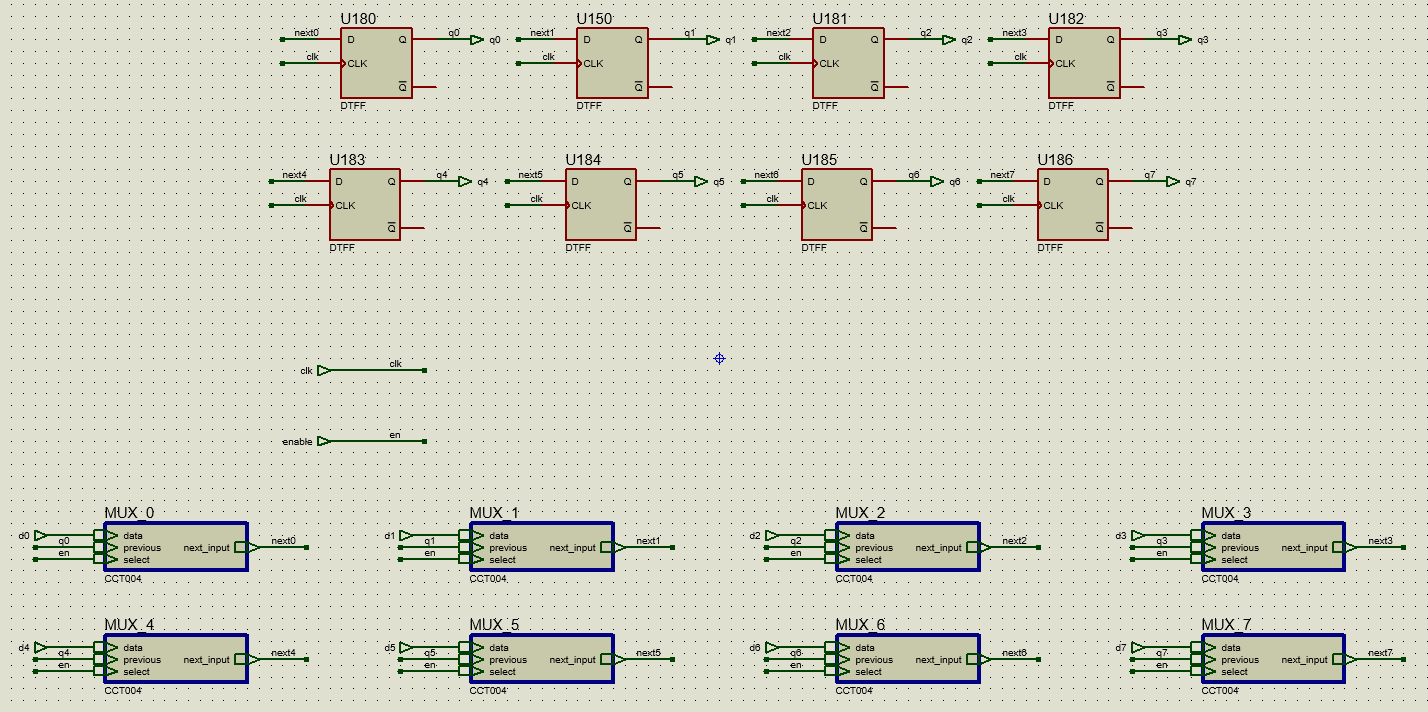
\includegraphics[width=0.6\textwidth]{source/is_inner.png}
		\caption{طراحی داخلی ماژول \lr{IR}}
		\label{fig:is-inner}
	\end{figure}
	
	\subsection{ماژول \lr{ALU}}
	بخش زیادی از این ماژول بدون تغییر از آزمایش‌های قبلی است. اما تعدادی ورودی و خروجی به آن اضافه شده است.
	\begin{figure}[H]
		\centering
		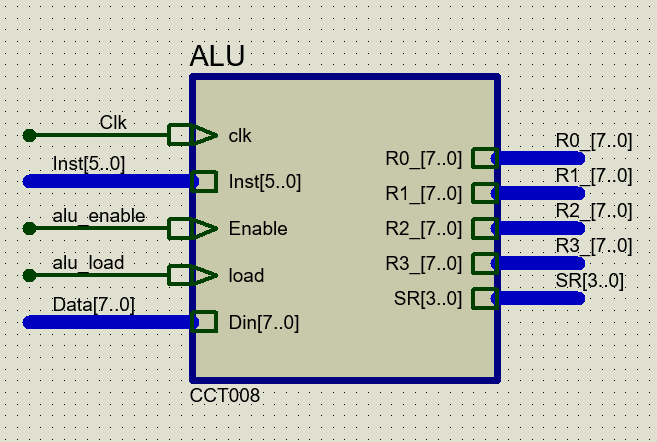
\includegraphics[width=0.5\textwidth]{source/alu_interface.png}
		\caption{ماژول \lr{ALU}}
		\label{fig:alu-interface}
	\end{figure}
	همانطور که در شکل \ref{fig:alu-interface} دیده می‌شود، ورودی‌های 
	\lr{Enable}
	،
	\lr{load}
	و
	\lr{Din}
	به ماژول اضافه شده‌اند که به ترتیب امکان خاموش کردن ماژول، بارگذاری در آن و داده‌ی ورودی به آن را به ما می‌دهند. با یک شدن سیگنال \lr{load} مقادیر \lr{Din} در رجیستر 
	\lr{R$_0$}
	ذخیره خواهد شد. هم‌چنان در دستورالعمل‌هایی که به واحد محاسبه نیازی نداریم، ورودی 
	\lr{Enable}
	این ماژول $0$ خواهد شد.
	
	تغییرات طراحی داخلی این ماژول نخست شامل ورودی رجیستر 
	\lr{R$_0$}
	است که به صورت زیر خواهد بود.
	\begin{figure}[H]
		\centering
		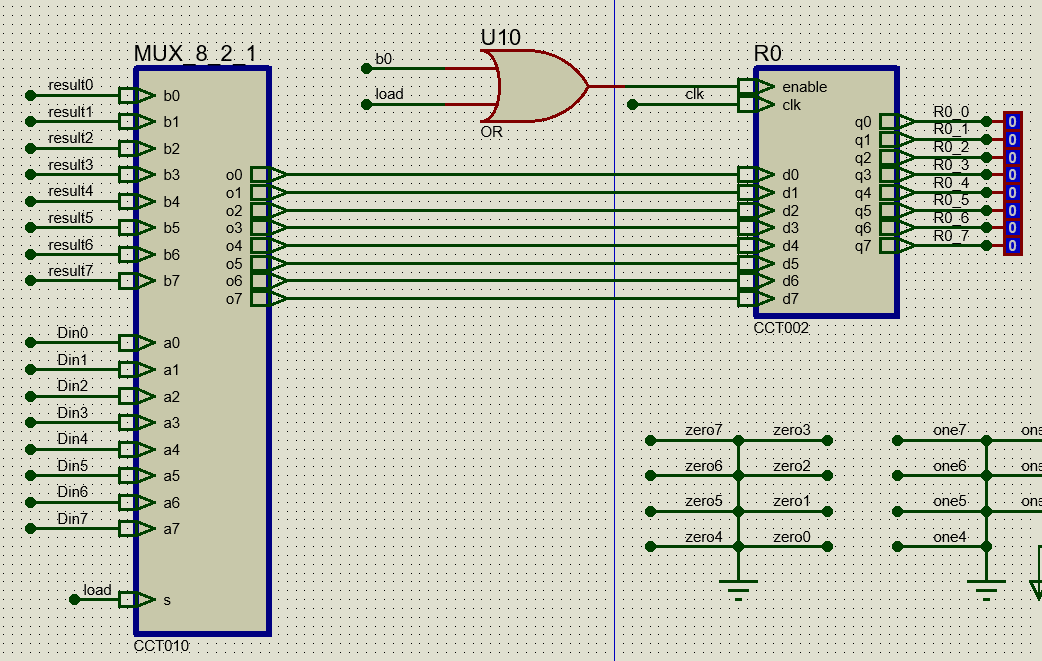
\includegraphics[width=0.68\textwidth]{source/alu1_inner.png}
		\caption{تغییرات طراحی داخلی \lr{ALU}}
		\label{fig:alu1-inner}
	\end{figure}
	همانطور که دیده می‌شود، ورودی این ماژول براساس سیگنال \lr{load} انتخاب می‌شود. هم‌چنین برای بررسی پرش‌های شرطی، به تعدادی \lr{flag} نیاز داشتیم که این \lr{flag}ها براساس نتیجه‌ی عملیات واحد محاسبه مشخص می‌شوند. برای افزودن این امکان به سیستم، مدار زیر به ماژول اضافه شده است.
	\begin{figure}[H]
		\centering
		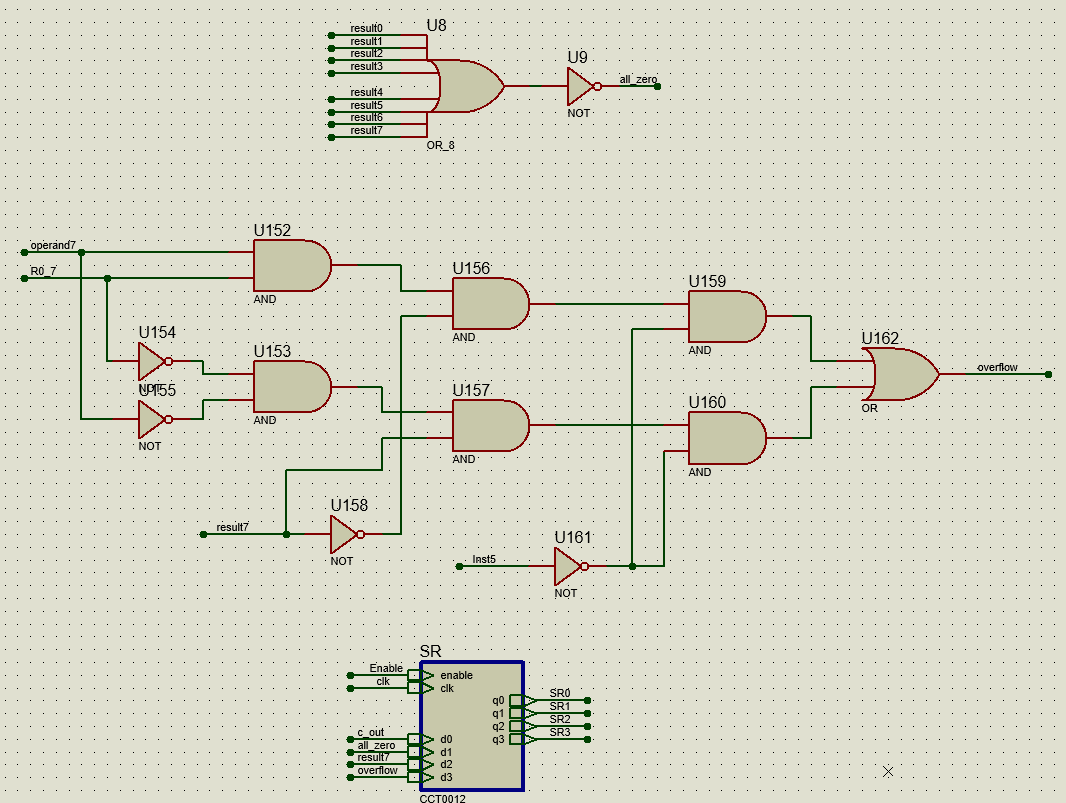
\includegraphics[width=0.68\textwidth]{source/sr.png}
		\caption{طراحی مدار برای \lr{SR}}
		\label{fig:sr-inner}
	\end{figure}
	برای بررسی صفر بودن کافیست مشابه تصویر \lr{OR} تمام بیت‌های حاصل صفر باشد. برای بررسی \lr{carry} که از خروجی \lr{carry} جمع‌کننده استفاده شده است. برای بررسی \lr{overflow} نیز از این واقعیت استفاده شده که اگر دو عدد مثبت را با یکدیگر جمع زده و حاصل منفی باشد، آن‌گاه \lr{overflow} رخ داده است. هم‌چنین با مثبت شدن جمع یا تفرق تو عدد منفی با یکدیگر نیز \lr{overflow} رخ داده است. از این توصیف همناطور که در تصویر دیده می‌شود برای تولید سیگنال \lr{overflow} استفاده شده است. ماژول \lr{SR} نیز یک رجیستر ۴بیتی است که این \lr{flag}ها را در خود نگه می‌دارد.
	
	\subsection{ماژول \lr{DATA\_MEM}}
	این ماژول به مدار اضافه شده تا بتوان مقادیر بینابینی را در حافظه‌ی سیستم ذخیره کرد و یا از آن این مقادیر را خواند. ورودی‌ها و خروجی‌های آن در شکل \ref{fig:datamem} آمده است.
	\begin{figure}[H]
		\centering
		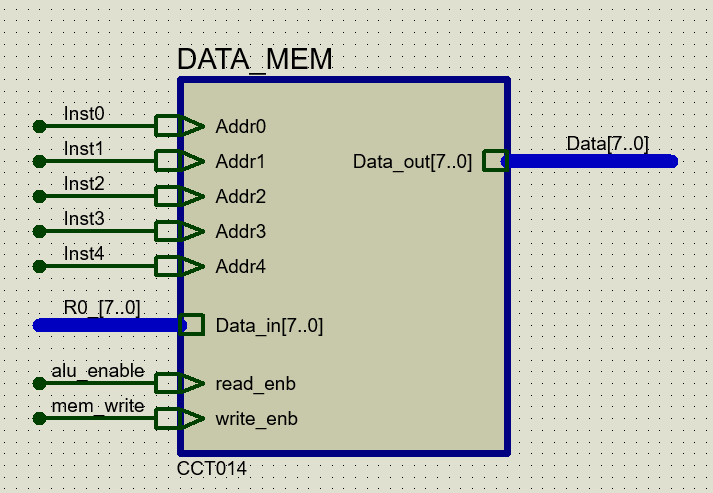
\includegraphics[width=0.45\textwidth]{source/datamem_interface.png}
		\caption{ماژول \lr{DATA\_MEM}}
		\label{fig:datamem}
	\end{figure}
	در طراحی داخلی این ماژول از تراشه‌ی \lr{6116} استفاده شده که یک \lr{RAM} شامل 32 بایت می‌شود. این تراشه هم قابلیت خواندن و هم قابلیت نوشتن را داراست. برای این منظور با استفاده از ترای استیت بافر داده‌ی ورودی را به تراشه داده یا داده‌ی خروجی آن را می‌خوانیم. طراحی مذکور در شکل \ref{fig:datamem_inner} آمده است.
	\begin{figure}[H]
		\centering
		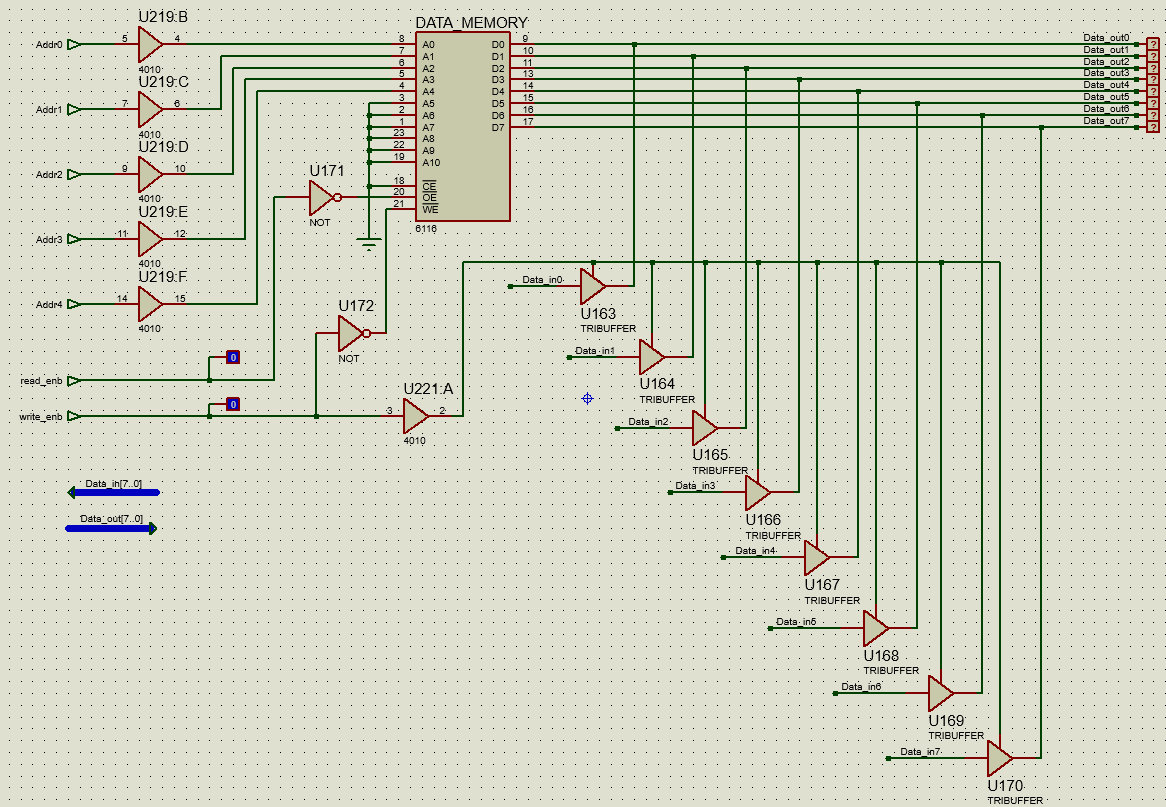
\includegraphics[width=0.75\textwidth]{source/datamem_inner.png}
		\caption{طراحی داخلی ماژول \lr{DATA\_MEM}}
		\label{fig:datamem_inner}
	\end{figure}
	
	\subsection{ماژول \lr{CU}}
	این ماژول همانطور که از نامش پیداست، وظیفه‌ی کنترل مدار را بر عهده دارد. به طور کلی سیگنال‌های مربوط به فعال شدن واحد محاسبه، خواندن یا نوشتن روی حافظه را تولید می‌کند. ورودی‌ها و خروجی‌های آن در شکل \ref{fig:cu_interface} آمده است.
	\begin{figure}[H]
		\centering
		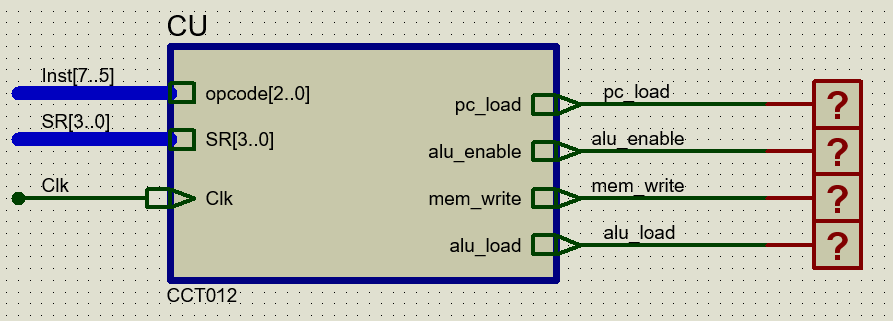
\includegraphics[width=0.45\textwidth]{source/cu_interface.png}
		\caption{ماژول \lr{CU}}
		\label{fig:cu_interface}
	\end{figure}
	برای ساخت سیگنال 
	\lr{pc\_load}
	از یک مالتی‌پلکسر ۴ به ۱ استفاده شده که براساس دستور ورودی و محتویات رجیستر \lr{SR}، تصمیم می‌گیرد که سیگنال مورد نظر باید 1 باشد یا 0. فلیپ‌فلاپ استفاده شده نیز به این منظور است که پس از یک شدن سیگنال \lr{pc\_load}، نهایتا در نیم‌کلاک بعد باید این سیگنال را خاموش کنیم تا در کلاک بعدی که دستورالعمل بعدی می‌آید، این دستورالعمل در \lr{PC} بارگذاری نشود.
	\begin{figure}[H]
		\centering
		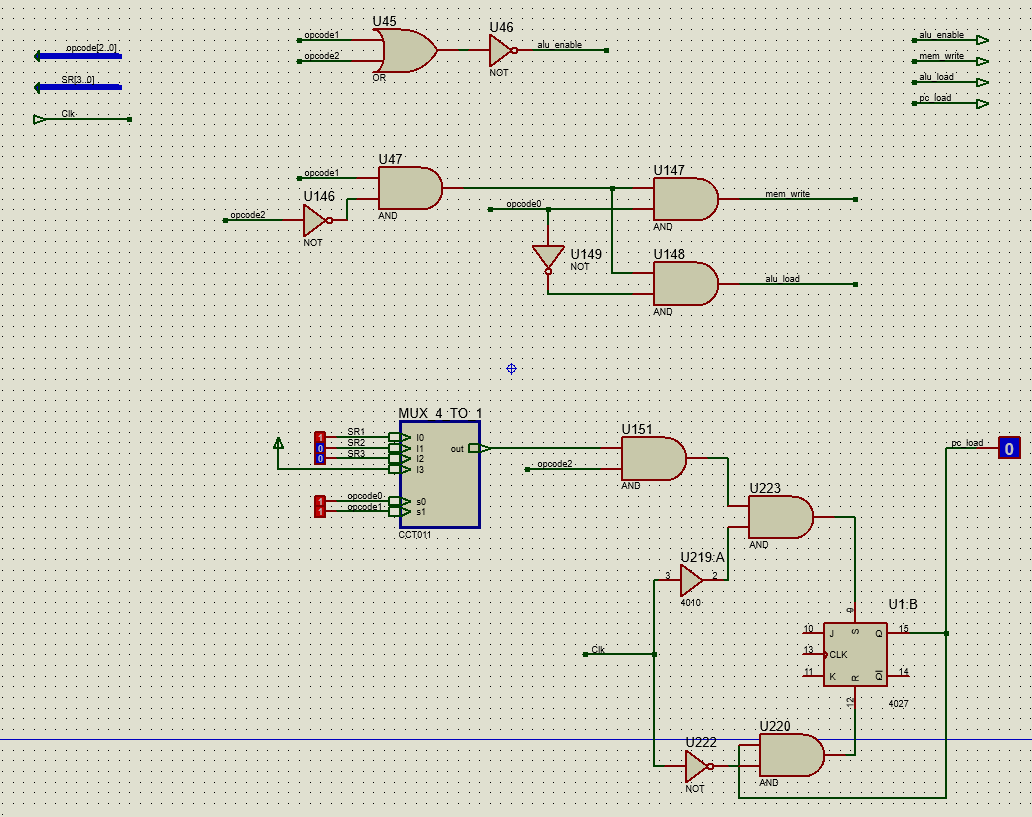
\includegraphics[width=0.75\textwidth]{source/cu_inner.png}
		\caption{طراحی داخلی ماژول \lr{CU}}
		\label{fig:cu_inner}
	\end{figure}
	ساخت سیگنال‌های
	\lr{mem\_write}
	،
	\lr{alu\_load}
	و
	\lr{alu\_enable}
	نیز به راحتی از روی بیت‌های دستورالعمل انجام شده است.
	%--------------------------------------------------
	\pagebreak
	\section{تست مدار}
	مطابق دستورالعمل، به منظور تست مدار مجموع 10 جمله‌ی اول دنباله‌ی فیبوناچی محاسبه شده است. کد ماشین و کد دستوری این برنامه به ترتیب در فایل‌های
	\lr{fibo\_machine.txt}
	و
	\lr{fibo\_code.txt}
	همراه فایل گزارش آمده است. خروجی سیستم پس از اجرای کامل این برنامه را نیز در شکل
	می‌توان مشاهده کرد.
	\begin{figure}[H]
		\centering
		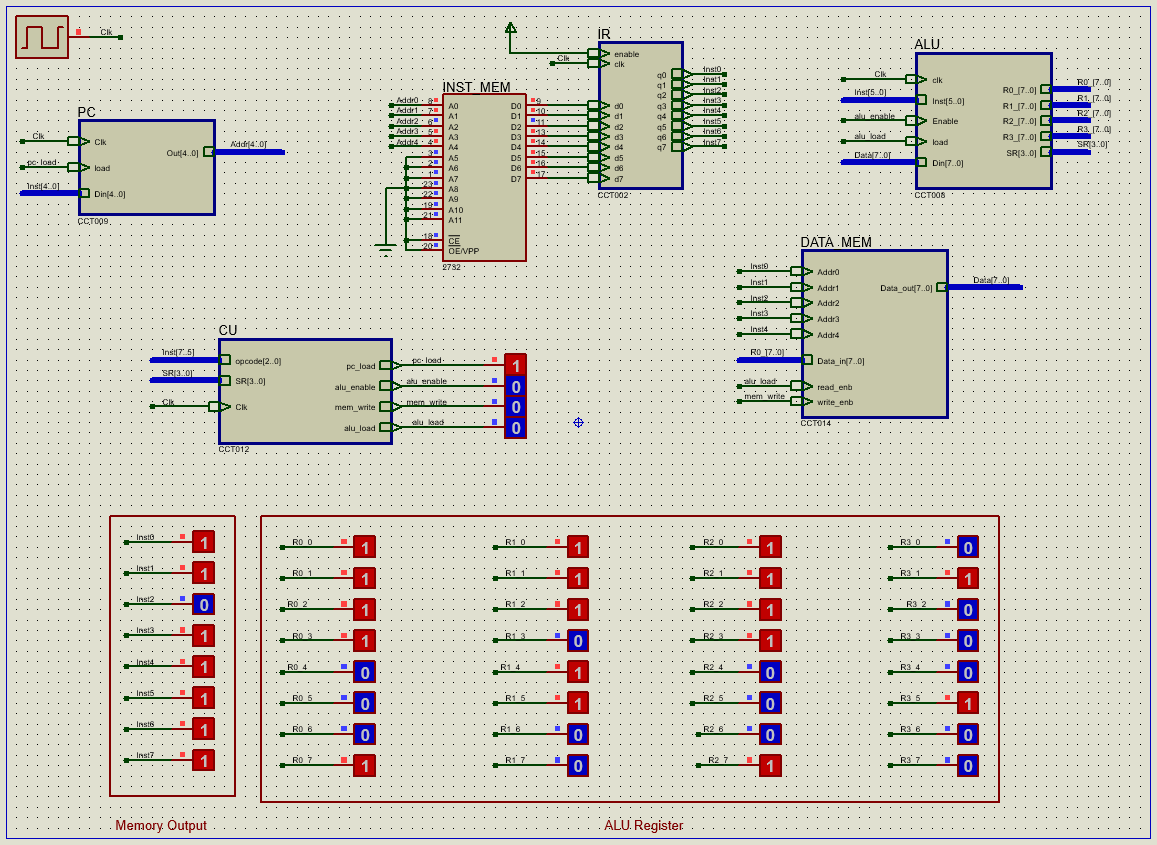
\includegraphics[width=0.9\textwidth]{source/fibo_final.png}
		\caption{وضعیت مدار پس از اجرای کامل برنامه‌ی \lr{fibo\_machine.bin}}
		\label{fig:fibo}
	\end{figure}
	در این برنامه رجیستر
	\lr{R$_2$}
	جمع مورد نظر را نگه‌داری می‌کرده است که در انتها برابر
	$(10001111)_2 = 2^7 + 8 + 4 + 2 + 1 = 143$
	شده است که برابر جمع 10 جمله‌ی اول دنباله فیبوناچی است.
\end{document}